\documentclass{ieeeaccess}
\usepackage{cite}
\usepackage{amsmath,amssymb,amsfonts,amsthm}
\usepackage{mathtools}
\usepackage{graphicx}
\usepackage{textcomp}
\usepackage[utf8]{inputenc}
\usepackage[T1]{fontenc}
\usepackage{bm}
\usepackage{algorithm}
\usepackage{algpseudocode}
\usepackage{booktabs}
\usepackage{xcolor}
\usepackage{hyperref}
\usepackage{multirow}
\usepackage{array}
\usepackage{tabularx}
\usepackage{subcaption}
\usepackage{enumitem}
\usepackage{cleveref}
\usepackage{siunitx}
\usepackage{bm}
\makeatletter
\AtBeginDocument{\DeclareMathVersion{bold}
\SetSymbolFont{operators}{bold}{T1}{times}{b}{n}
\SetSymbolFont{NewLetters}{bold}{T1}{times}{b}{it}
\SetMathAlphabet{\mathrm}{bold}{T1}{times}{b}{n}
\SetMathAlphabet{\mathit}{bold}{T1}{times}{b}{it}
\SetMathAlphabet{\mathbf}{bold}{T1}{times}{b}{n}
\SetMathAlphabet{\mathtt}{bold}{OT1}{pcr}{b}{n}
\SetSymbolFont{symbols}{bold}{OMS}{cmsy}{b}{n}
\renewcommand\boldmath{\@nomath\boldmath\mathversion{bold}}}
\makeatother

\def\BibTeX{{\rm B\kern-.05em{\sc i\kern-.025em b}\kern-.08em
    T\kern-.1667em\lower.7ex\hbox{E}\kern-.125emX}}

% ── Theorem-like environments ──────────────────────────────────────────
\newtheorem{remark}{Remark}

% ── Math shorthands ────────────────────────────────────────────────────
\newcommand{\R}{\mathbb{R}}
\newcommand{\norm}[1]{\left\| #1 \right\|}
\newcommand{\vect}[1]{\bm{#1}}
\newcommand{\mat}[1]{\mathbf{#1}}
\newcommand{\dt}{\Delta t}
\newcommand{\st}{\text{s.t.}}
\newcommand{\pmm}{\textsc{pmm}}
\newcommand{\nmpc}{\textsc{nmpc}}
\newcommand{\mujoco}{MuJoCo}

%Your document starts from here _______________________________________________
\begin{document}
\history{Date of publication xxxx 00, 0000, date of current version xxxx 00, 0000.}
\doi{10.1109/ACCESS.2025.0000000}

\title{Point Mass Planning and NMPC Tracking for
       Time-Optimal Agile Quadrotor Gate Navigation}

\author{{Bryan S. Guevara}\authorrefmark{1},
and José Varela-Aldás\authorrefmark{1},~\IEEEmembership{Senior Member, IEEE}}

\address[1]{Centro de Investigación MIST, Facultad de Ingenierías,
Universidad Tecnológica Indoamérica, \mbox{Ambato 180103}, Ecuador
(e-mail: bguevara@indoamerica.edu.ec; josevarela@uti.edu.ec)}

\tfootnote{The research was funded by Universidad Indoamérica.}

\markboth
{B. S. Guevara \headeretal:~Point Mass Planning and NMPC Tracking for Agile Gate Navigation}
{B. S. Guevara \headeretal:~Point Mass Planning and NMPC Tracking for Agile Gate Navigation}

\corresp{Corresponding author: José Varela-Aldás (e-mail: josevarela@uti.edu.ec).}

\begin{abstract}
Time-optimal agile flight through a sequence of three-dimensional gates
requires a consistent coupling between trajectory planning and tracking
control.
Point-mass planners offer fast numerical solutions for free-final-time
optimisation, but the value of progressively enriching the reference fed
to a nonlinear model predictive control (\nmpc{}) tracker through a
differential flatness bridge has not been clearly characterised on
multi-gate circuits.
This paper presents a modular three-stage pipeline: an offline
time-optimal point-mass model (\pmm{}) planner solved with CasADi and
IPOPT; a differential flatness bridge that maps the flat outputs and
their time derivatives to a full quadrotor reference comprising desired
position, velocity, attitude quaternion, body angular rate, and
collective thrust; and a body-rate \nmpc{} tracker implemented on the
acados SQP-RTI scheme with an SO(3) logarithmic-map external cost.
Two reference configurations are compared in a software-in-the-loop
setup that drives the \mujoco{} physics engine through ROS~2 under a
randomly seeded external-force disturbance.
The baseline, \nmpc{}-Att, uses only a yaw-only attitude reference
derived from the velocity heading and carries no angular-rate or thrust
feedforward.
The proposed configuration, \nmpc{}-Full, activates the complete flat
reference, including the full attitude quaternion, body angular rate,
and thrust feedforward.
Results on a seven-gate figure-8 and an eight-gate vertical loop show
that reference enrichment yields a categorical improvement in gate
crossing and a systematic reduction of tracking error without increasing
solver cost.
The loop circuit further highlights a structural limitation of the
common practice yaw-only reference: it cannot represent inverted
attitudes, and only the flatness-based reference resolves this case.
\end{abstract}

\begin{keywords}
Agile flight, differential flatness, gate navigation, model predictive
control, nonlinear control, point mass model, quadrotor UAV,
time-optimal planning.
\end{keywords}

\titlepgskip=-21pt

\maketitle

% ==========================================================================
\section{Introduction}
\label{sec:introduction}
% ==========================================================================

\PARstart{A}{gile} quadrotor flight through a sequence of three-dimensional
gates is a challenging benchmark in autonomous aerial robotics.
In state-of-the-art racing systems, gate navigation drives the vehicle
near its actuation limits, with reported peak accelerations in excess
of $4g$ and peak speeds above 60~km/h while respecting geometric passage
constraints~\cite{foehn2021time,romero2022mpcc,kaufmann2023champion}.
Model-based approaches decompose this task into a planner and a tracker,
coupled through an intermediate reference trajectory~\cite{song2023reaching}.
A central design question in this coupling is how much of the
planner output should be communicated to the tracker: a position-only
reference is simple to compute, while a full flatness-derived reference
requires inverting the differential flatness map but carries attitude,
angular rate, and thrust information that the tracker would otherwise
have to reconstruct from error feedback alone.
The quantitative effect of this choice on gate-crossing performance has
received limited study in multi-gate scenarios.

\subsection{Related Work}
\label{subsec:related}

Time-optimal planning for agile flight has converged on two families.
Polynomial-flatness approaches following Mellinger and
Kumar~\cite{mellinger2011minimum} cast trajectory generation as a
quadratic program over piecewise segments and recover attitude and
angular-rate references from flat outputs, but they are smooth rather
than time-optimal and rely on separate time
allocation~\cite{richter2016polynomial,mellinger2012trajectory}.
Point-mass formulations relax rotational dynamics to expose the
translational time-optimality structure:
Mueller~\textit{et~al.}~\cite{mueller2015computationally} derived
closed-form \pmm{} primitives between full kinematic states;
Foehn~\textit{et~al.}~\cite{foehn2021time} extended this to multi-waypoint
flight via Complementary Progress Constraints solved with IPOPT and
matched expert pilot times; and the TOGT planner of
Qin~\textit{et~al.}~\cite{qin2024togt} incorporated explicit gate
geometry and single-rotor thrust bounds, solving nine-gate circuits in
seconds.
Related minimum-time formulations extend to cluttered
environments~\cite{penicka2022minimum}.
Across this family, trajectory quality is high but the tracking problem
is left open.

Learning-based methods close the tracking loop by sidestepping the
reference entirely.
Loquercio~\textit{et~al.}~\cite{loquercio2021learning} trained a deep
policy for 40~km/h flight in unstructured environments; the Swift
system~\cite{kaufmann2023champion} reached world-champion-level racing
using deep reinforcement learning; and
Song~\textit{et~al.}~\cite{song2023reaching} showed that reinforcement
learning can outperform optimal control by directly optimising the
task-level objective, identifying the plan-then-track interface itself
as a principal performance limit of model-based pipelines.
The present work targets this interface from the opposite direction,
enriching its content while preserving modularity.

Nonlinear model predictive control has become the dominant model-based
tracker because the body-rate formulation
\cite{hanover2021performance} retains attitude-dependent coupling while
delegating fast rate dynamics to an inner loop, and because real-time
solvers such as acados with
SQP-RTI~\cite{verschueren2022acados,diehl2005real} deliver
sub-millisecond QPs at 100~Hz.
Robustness has been addressed by cascading \nmpc{} with an L1 adaptive
controller under unknown payload and wind
\cite{hanover2021performance}, by augmenting with a Gaussian-process
aerodynamic residual~\cite{torrente2021datadriven}, and by incremental
nonlinear dynamic inversion with flatness
feedforward~\cite{tal2021accurate}; ROS-based MPC baselines for UAV
trajectory tracking are widely available~\cite{kamel2017model}.
The benchmark comparison by Sun~\textit{et~al.}~\cite{sun2022comparative}
against differential-flatness-based control over 76 trajectories
establishes \nmpc{} superiority for dynamically infeasible references
but fixes the reference structure and does not ablate its components.

Model Predictive Contouring Control fuses planning and tracking in a
single online optimisation that maximises path progress while
minimising contouring error~\cite{romero2022mpcc}, and recent variants
add \pmm{}-based online replanning around moving
gates~\cite{romero2022replanning} and tunnel-based safety constraints
that reach 100\% crossing success above
80~km/h~\cite{krinner2024mpcc}; perception-latency bounds for
high-speed flight are characterised by
Falanga~\textit{et~al.}~\cite{falanga2018how}.
MPCC performance is strong, but its planner and controller cannot be
independently designed, validated, or replaced.

As a planning-control bridge, differential flatness was established for
quadrotors in~\cite{mellinger2011minimum} and extended to rotor-drag
models in~\cite{faessler2018differential}, yielding algebraic maps from
position and heading and their time derivatives to thrust, attitude,
and body-rate references~\cite{faessler2017thrust}.
Greeff and Schoellig~\cite{greeff2018flatness} integrated flatness
feedforward into a linearised MPC, and
Sun~\textit{et~al.}~\cite{sun2022comparative} used flatness-derived
references for both \nmpc{} and DFBC without varying the reference
components.
A common practical compromise in \nmpc{} design is to derive only a
desired yaw angle from the trajectory planner
($\psi^*=\mathrm{atan2}(v_y,v_x)$) and convert it to a quaternion
reference, while omitting the angular-rate and thrust feedforward that
a full flatness inversion would provide.
No prior work quantifies the performance gap between this common-practice
incomplete reference and the complete flat output
$(\vect{p},\vect{v},\vect{q},\vect{\omega},T)$ on a multi-gate 3D
circuit.

Across these three families, three patterns recur: (i) PMM and TOGT
planners deliver strong time-optimal references but do not specify
how much of the flat output the tracker consumes; (ii) body-rate
\nmpc{} trackers have been benchmarked with fixed reference structures
and without a gate-navigation objective; and (iii) MPCC fuses the two
stages at the cost of modularity.
No prior study decouples planner and tracker via a full flatness
bridge and ablates the reference content on a multi-gate 3-D circuit
under identical dynamics, solver, and cost; this is the gap addressed
here.

\subsection{Identified Gap}
\label{subsec:gap}

Two related gaps motivate this study.
\emph{First}, a pipeline that combines an offline \pmm{} planner, a
differential flatness bridge, and a body-rate \nmpc{} tracker receiving
the full flat reference has not, to our knowledge, been reported as an
integrated system in this specific form.
Foehn~\textit{et al.}~\cite{foehn2021time} combine \pmm{} with \mbox{MPCC}
tracking but without a flatness-derived full-state reference fed to an
\nmpc{}.
\mbox{TOGT}~\cite{qin2024togt} is a planner-only contribution.
\emph{Second}, existing studies of \nmpc{} for agile flight typically fix
the reference structure.
The performance difference between the common-practice incomplete attitude
reference (yaw derived from velocity direction) and the full flatness
inversion has not been isolated on a multi-gate circuit under otherwise
identical dynamics, solver, and cost structure.
Identifying this difference precisely is necessary to justify the
additional computation of the full flatness bridge.

\subsection{Contributions}
\label{subsec:contributions}

The contributions of this paper are:

\begin{enumerate}

\item \textbf{Integrated \pmm{}--flatness--\nmpc{} pipeline.}
      A modular architecture coupling an offline \pmm{} planner
      (CasADi + IPOPT), a differential flatness bridge that maps the
      flat outputs to a 17-component quadrotor reference, and a
      body-rate \nmpc{} tracker (acados SQP-RTI, $N=50$, \SI{100}{\hertz})
      with an SO(3) logarithmic-map external cost.

\item \textbf{Flatness-inversion benefit on multi-gate circuits.}
      A \mujoco{} software-in-the-loop evaluation on a figure-8 and a
      vertical loop with inverted apex shows that the angular-rate
      feedforward is the dominant factor for gate-crossing at
      aggressive rotational transitions, and that the tilt-corrected
      quaternion is necessary for the \emph{feasibility} of inverted
      segments that the yaw-only reference cannot represent by
      construction.

\end{enumerate}

\subsection{Paper Organization}
\label{subsec:organization}

Section~\ref{sec:model} introduces the body-rate quadrotor model and
the notation used throughout the paper.
Section~\ref{sec:pmm} formulates the time-optimal gate navigation
problem and details the \pmm{} planner.
Section~\ref{sec:flatness} derives the differential flatness bridge.
Section~\ref{sec:nmpc} formulates the \nmpc{} tracker.
Section~\ref{sec:results} defines the two reference configurations,
describes the \mujoco{} evaluation, and reports the results.
Section~\ref{sec:conclusion} concludes the paper.

% ==========================================================================
\section{Quadrotor Model}
\label{sec:model}
% ==========================================================================

The quadrotor is modelled at the body-rate level, delegating low-level
attitude dynamics to an inner-loop rate controller, as is standard for
agile \nmpc{}~\cite{hanover2021performance}.
The state
$\vect{x}=[\vect{p}^\top,\vect{v}^\top,\vect{q}^\top,
          \vect{\omega}^\top]^\top\in\R^{13}$
collects the position $\vect{p}$ and linear velocity $\vect{v}$,
expressed in the world frame $\mathcal{W}$ (with
$\vect{e}_3=[0,0,1]^\top$ aligned with gravity);
the attitude quaternion
$\vect{q}=[q_w,q_x,q_y,q_z]^\top\in\mathbb{S}^3$ in Hamilton convention,
representing the rotation from the body frame $\mathcal{B}$ to
$\mathcal{W}$ and inducing the rotation matrix
$\mat{R}(\vect{q})\in SO(3)$; and the body angular velocity
$\vect{\omega}$ expressed in $\mathcal{B}$.
The control input
$\vect{u}=[T,\,\omega_x^c,\,\omega_y^c,\,\omega_z^c]^\top$
consists of the collective thrust $T\geq 0$ along $\vect{z}_\mathcal{B}$
and the commanded body angular rate $\vect{\omega}^c$.
The continuous-time dynamics are
%
\begin{align}
  \dot{\vect{p}} &= \vect{v}, \label{eq:dyn_p} \\
  \dot{\vect{v}} &= -g\,\vect{e}_3
                    + \frac{T}{m}\,\mat{R}(\vect{q})\,\vect{e}_3,
                    \label{eq:dyn_v} \\
  \dot{\vect{q}} &= \tfrac{1}{2}\,\mat{\Xi}(\vect{q})\,\vect{\omega},
                    \label{eq:dyn_q} \\
  \dot{\vect{\omega}} &= \frac{\vect{\omega}^c - \vect{\omega}}{\tau_{rc}},
                    \label{eq:dyn_w}
\end{align}
%
with vehicle mass $m$, gravitational acceleration $g$, and first-order
rate-controller time constant $\tau_{rc}$.
The kinematic matrix $\mat{\Xi}(\vect{q})$ in~\eqref{eq:dyn_q} is the
standard Hamilton form~\cite{mellinger2011minimum}; the unit-norm
constraint $\norm{\vect{q}}=1$ is preserved by renormalising $\vect{q}$
after each integration step.
Model~\eqref{eq:dyn_p}--\eqref{eq:dyn_w} serves as the prediction model
of the \nmpc{} (Section~\ref{sec:nmpc}) and as the substrate onto which
the differential flatness map (Section~\ref{sec:flatness}) inverts the
planner output.

% ==========================================================================
\section{Point Mass Time-Optimal Planner}
\label{sec:pmm}
% ==========================================================================

\subsection{Time-Optimal Gate Navigation Problem}
\label{sec:prob}

Let
$\mathcal{G}=\{(\vect{g}_i,\hat{\vect{n}}_i,r_i)\}_{i=1}^{N_g}$
denote a sequence of $N_g$ gates, each defined by centre position
$\vect{g}_i\in\R^3$, unit normal $\hat{\vect{n}}_i$, and radius $r_i$.
The time-optimal gate navigation problem seeks a trajectory that
minimises the final time~$T_f$ subject to the quadrotor
dynamics~\eqref{eq:dyn_p}--\eqref{eq:dyn_w}, actuator bounds on the
collective thrust and body rate, and, for each gate $i=1,\ldots,N_g$, a
crossing instant $t_i\in[0,T_f]$ at which the vehicle pierces the gate
plane within its radius:
%
\begin{align}
  \hat{\vect{n}}_i^\top(\vect{p}(t_i)-\vect{g}_i) &= 0,
  \label{eq:gate_plane}\\
  \norm{\vect{p}(t_i)-\vect{g}_i}_\perp &\leq r_i-\delta,
  \label{eq:gate_radius}
\end{align}
%
where $\norm{\cdot}_\perp$ denotes the in-plane distance to the gate
centre and $\delta>0$ is a safety margin.
Solving this problem directly on the full 13-dimensional
model~\eqref{eq:dyn_p}--\eqref{eq:dyn_w} with a free final time and
$N_g$ implicit crossing events is computationally challenging
\cite{foehn2021time}.
We therefore adopt a point-mass relaxation, which enables fast
offline solution and still captures the translational structure that
dominates gate-crossing timing; the flatness-based tracker of
Section~\ref{sec:flatness} subsequently reintroduces the attitude and
body-rate content that the relaxation discards.

\subsection{Point Mass Model}
\label{sec:pmm_model}

The \pmm{} approximates the quadrotor as a point mass with state
$\vect{s}=[\vect{p}^\top,\vect{v}^\top]^\top\in\R^6$ and control
$\vect{a}\in\R^3$ (desired acceleration):
\begin{equation}
  \dot{\vect{s}}=
  \begin{bmatrix}\vect{v}\\\vect{a}\end{bmatrix}.
  \label{eq:pmm_dyn}
\end{equation}
Attitude dynamics are abstracted away; this relaxation is valid when
the rate-loop settling time $\tau_{rc}$ in~\eqref{eq:dyn_w} is small
relative to the collocation step $T_f/N$ used below.

\subsection{NLP Formulation}
\label{sec:pmm_nlp_formulation}

The continuous problem is transcribed via direct multiple shooting with
$N_\text{PMM}$ collocation steps and free final time $T_f$.
The variable step size $\dt = T_f/N_\text{PMM}$ couples the time horizon
to $T_f$:
%
\begin{subequations}
\label{eq:pmm_nlp}
\begin{align}
  \min_{\vect{S}, \vect{A}, T_f}\;&
     w_T\,T_f
     + w_a \sum_{k=0}^{N_\text{PMM}-1} \norm{\vect{a}_k}^2 \dt
     + w_j \sum_{k=1}^{N_\text{PMM}-1}
       \frac{\norm{\vect{a}_k - \vect{a}_{k-1}}^2}{\dt}
     \label{eq:pmm_cost}\\
  \st\quad & \vect{s}_{k+1} = \mathrm{RK4}(\vect{s}_k, \vect{a}_k, \dt),
     \label{eq:pmm_dyn_c}\\
  & \vect{s}_0 = \vect{s}_\text{init},\quad
              \vect{s}_{N_\text{PMM}} = \vect{s}_\text{final},
              \label{eq:pmm_bc}\\
  & \hat{\vect{n}}_i^\top (\vect{p}_{k_i} - \vect{g}_i) = 0,\quad
    \norm{\vect{p}_{k_i} - \vect{g}_i}_\perp \leq r_i - \delta,
              \label{eq:pmm_gate}\\
  & d_i^- < 0 < d_i^+, \quad i = 1,\dots,N_g,
              \label{eq:pmm_crossing}\\
  & \norm{\vect{v}_k} \leq v_{\max},\quad
              \norm{\vect{a}_k} \leq a_{\max},\quad T_f \geq T_{\min},
              \label{eq:pmm_bounds}
\end{align}
\end{subequations}
%
where $d_i^{\pm} = \hat{\vect{n}}_i^\top(\vect{p}_{k_i \pm 1} - \vect{g}_i)$
enforce the correct approach direction through each
gate~\eqref{eq:pmm_crossing}.
The NLP is formulated with CasADi~\cite{andersson2019casadi} and solved
offline with IPOPT~\cite{wachter2006implementation}.

% ==========================================================================
\section{Differential Flatness Reference Conversion}
\label{sec:flatness}
% ==========================================================================

\subsection{Flat Output and Dependency Structure}
\label{sec:flat_output}

The quadrotor is differentially flat with flat output
$\vect{\sigma}=[\vect{p}^\top,\psi]^\top\in\R^4$, the position in
$\mathcal{W}$ together with the yaw angle~$\psi$
\cite{mellinger2011minimum,faessler2018differential}.
Flatness means that every state and input component of the body-rate
model~\eqref{eq:dyn_p}--\eqref{eq:dyn_w} can be expressed as an algebraic
function of $\vect{\sigma}$ and a finite number of its time derivatives,
without integration of the dynamics.
For the body-rate model used here, the dependency chain reads
$\vect{v}=\dot{\vect{p}}$;
the specific force $\vect{f}=\ddot{\vect{p}}+g\,\vect{e}_3$ yields the
collective thrust $T=m\norm{\vect{f}}$ and the body $z$-axis
$\vect{z}_B=\vect{f}/\norm{\vect{f}}$; the remaining two body axes are
fixed by $\psi$, producing the rotation matrix $\mat{R}$ and hence the
quaternion $\vect{q}$; and the body angular velocity $\vect{\omega}$ is
the axial vector of $\mat{R}^\top\dot{\mat{R}}$.
In this pipeline the \pmm{} planner does not produce an independent yaw
reference, so $\psi$ is fixed by the downstream convention specified
in Section~\ref{sec:flat_map}.
One departure from the closed-form flatness maps
of~\cite{mellinger2011minimum,faessler2018differential} is that the
angular velocity $\vect{\omega}^*$ is computed via numerical forward
finite difference of the discrete rotation sequence rather than
analytically from position jerk; this choice is motivated in
Section~\ref{sec:flat_map}.

\subsection{From PMM Outputs to Full Quadrotor Reference}
\label{sec:flat_map}

The \pmm{} supplies position, velocity, and acceleration on the
collocation grid; jerk is recovered by backward finite differences,
$\vect{j}_k\approx(\vect{a}_k-\vect{a}_{k-1})/\dt^*$, and these
translational quantities determine the remaining degrees of freedom of
the quadrotor state through the chain laid out below.
Newton's second law identifies the specific force
$\vect{f}^*=\vect{a}+g\,\vect{e}_3$, from which the collective thrust and
the body $z$-axis follow directly:
\begin{equation}
  T^*=m\,\norm{\vect{f}^*},\qquad
  \vect{z}_B^*=\frac{\vect{f}^*}{\norm{\vect{f}^*}}.
  \label{eq:T_des}
\end{equation}
The remaining two body axes are fixed by the yaw convention
$\psi^*=\mathrm{atan2}(v_y,v_x)$ with heading vector
$\vect{x}_C=[\cos\psi^*,\sin\psi^*,0]^\top$, giving
\begin{align}
  \vect{y}_B^* &= \frac{\vect{z}_B^*\times\vect{x}_C}
                        {\norm{\vect{z}_B^*\times\vect{x}_C}},\qquad
  \vect{x}_B^* = \vect{y}_B^*\times\vect{z}_B^*,\nonumber\\
  \mat{R}^* &= \bigl[\,\vect{x}_B^*\;\big|\;\vect{y}_B^*\;\big|\;
               \vect{z}_B^*\,\bigr].
  \label{eq:R_des}
\end{align}
The body $z$-axis in~\eqref{eq:T_des} is undefined only if the specific
force vanishes, $\vect{a}=-g\vect{e}_3$, corresponding to pure
free-fall; this configuration is never realised by the \pmm{} output on
the eight-gate circuit.
The rotation matrix is converted to a unit quaternion with the
Shepperd method~\cite{shepperd1978quaternion}, whose pivot
$m=\arg\max\{1+\mathrm{tr}\mat{R}^*,\,1+2R_{11}-\mathrm{tr},\,
             1+2R_{22}-\mathrm{tr},\,1+2R_{33}-\mathrm{tr}\}$
maximises numerical conditioning across the four branch formulas; to
keep the discrete sequence on the same hemisphere of the double cover
$\vect{q}\sim-\vect{q}$, a consecutive pair with negative inner product
is flipped,
\begin{equation}
  \vect{q}_k^{*\top}\vect{q}_{k-1}^*<0
  \;\Rightarrow\;
  \vect{q}_k^*\leftarrow-\vect{q}_k^*.
  \label{eq:hemisphere}
\end{equation}
Differentiating $\mat{R}^*$ numerically then yields the body angular
velocity.
Because $\mat{R}^*$ is available only at the discrete collocation
nodes, the identity $[\vect{\omega}^*]_\times=\mat{R}^{*\top}\dot{\mat{R}}^*$
is evaluated with a forward finite difference,
\begin{equation}
  \dot{\mat{R}}_k^*\approx\frac{\mat{R}_{k+1}^*-\mat{R}_k^*}{\dt_k},
  \label{eq:Rdot}
\end{equation}
and the angular velocity is extracted from
$\mat{\Omega}_k=\mat{R}_k^{*\top}\dot{\mat{R}}_k^*$ via the vee map
$\vect{\omega}_k^*=\mat{\Omega}_k^\vee$.
The closed-form jerk-based angular-rate formula of Faessler~\textit{et
al.}~\cite{faessler2018differential} is not applicable here because it
requires continuous jerk, whereas the \pmm{} delivers only a
piecewise-constant acceleration on a non-uniform grid; for the same
reason, finite differencing on a variable step $\dt_k$ amplifies
high-frequency content, which we attenuate in two steps.
A causal 5-point uniform moving average,
$\bar{\omega}_{i,k}^*=\tfrac{1}{5}\sum_{j=0}^{4}\omega_{i,k-j}^*$, first
removes the differentiation noise while preserving the mean trend, and
a subsequent hard saturation $|\bar{\omega}_i^*|\leq\omega_{\max}^{\rm ref}
<\omega_{\max}$ reserves a small headroom below the actuator limit for
closed-loop corrections.
The resulting full state reference and thrust feedforward
\begin{equation}
  \vect{x}^*=
  \bigl[\vect{p}^{*\top},\vect{v}^{*\top},\vect{q}^{*\top},
        \vect{\omega}^{*\top}\bigr]^\top,\qquad
  u_\text{ff}=T^*,
  \label{eq:full_ref}
\end{equation}
are interpolated from the \pmm{} collocation grid to the \nmpc{}
sampling grid using not-a-knot cubic splines, completing the algebraic
bridge that an \nmpc{} tracker can consume in full.

% ==========================================================================
\section{NMPC Formulation}
\label{sec:nmpc}
% ==========================================================================

\subsection{Stage and Terminal Costs}
\label{sec:stage_cost}

The \nmpc{} receives reference information through a 17-component
parameter vector,
\begin{equation}
  \vect{p}_j=
  [\vect{p}_j^{*\top},\vect{v}_j^{*\top},
   \vect{q}_j^{*\top},\vect{\omega}_j^{*\top},
   T_j^*,\vect{0}_3^\top]^\top,
  \label{eq:param_vec}
\end{equation}
whose components are filled by the flatness bridge to the extent
appropriate for each reference configuration
(Section~\ref{sec:configurations}).
Because the attitude component lives on $SO(3)$, the cost measures
attitude error as a geodesic distance on the manifold rather than as a
Euclidean difference in quaternion coordinates; a raw quaternion
difference is discontinuous under the double cover $\vect{q}\sim-\vect{q}$
and destabilises the Gauss-Newton Hessian used by SQP-RTI.
We adopt the logarithmic map on $SO(3)$~\cite{lee2010geometric}.
Denoting the body-frame error quaternion
$\vect{q}_e=\vect{q}^{-1}\otimes\vect{q}^*$ with vector part
$\vect{q}_{e,v}=[q_{e,x},q_{e,y},q_{e,z}]^\top$ and, to restrict the
shortest-rotation branch, the sign convention $q_{e,w}\geq 0$
enforced by flipping $\vect{q}_e\leftarrow-\vect{q}_e$ when
$q_{e,w}<0$, the attitude error used in the cost is
\begin{equation}
  \vect{e}_R=\log_{SO(3)}(\vect{q}_e)
   =\frac{2\,\mathrm{atan2}(\norm{\vect{q}_{e,v}},\,q_{e,w})}
         {\norm{\vect{q}_{e,v}}+\varepsilon}\,\vect{q}_{e,v},
  \label{eq:log_so3}
\end{equation}
with a fixed regularisation $\varepsilon=10^{-9}$ that guarantees a
finite Gauss-Newton Hessian at $\vect{q}^*=\vect{q}$ without branching,
as required by the external-cost interface of acados.

The general stage cost penalises position, velocity, attitude,
angular-rate, and input deviations from the reference,
\begin{align}
  \ell =\;
    &\norm{\vect{p}^*-\vect{p}}_{\mat{Q}_p}^2
    + \norm{\vect{v}^*-\vect{v}}_{\mat{Q}_v}^2
    + \norm{\vect{e}_R}_{\mat{Q}_q}^2 \nonumber\\
    &+\norm{\vect{\omega}^*-\vect{\omega}}_{\mat{Q}_\omega}^2
    + \norm{\vect{u}-\vect{u}_\text{ff}}_{\mat{R}}^2,
  \label{eq:stage_cost}
\end{align}
with $\vect{e}_R$ from~\eqref{eq:log_so3}, diagonal positive-semidefinite
weights $\mat{Q}_p,\mat{Q}_v,\mat{Q}_q,\mat{Q}_\omega,\mat{R}$, and
control feedforward $\vect{u}_\text{ff}=[T^*,0,0,0]^\top$.
The terminal cost $V_f$ has the same form without the $\mat{R}$ term.
Not all weight matrices are active in every configuration: setting
$\mat{Q}_\omega=\mat{0}$ for \nmpc{}-Att drops the angular-rate term
entirely, which is the correct choice when no meaningful $\vect{\omega}^*$
reference is available, as detailed in Section~\ref{sec:configurations}.
Numerical values of the non-zero weights appear in
Section~\ref{sec:setup}.

\subsection{Optimal Control Problem}
\label{sec:ocp}

At each sampling instant $t_k$ the \nmpc{} solves the finite-horizon
problem
%
\begin{subequations}
\label{eq:ocp}
\begin{align}
  \min_{\vect{u}_{0:N-1}}\;&
     \sum_{j=0}^{N-1}\ell(\vect{x}_j,\vect{u}_j,\vect{p}_j)
     + V_f(\vect{x}_N,\vect{p}_N), \label{eq:ocp_cost}\\
  \st\quad & \vect{x}_{j+1}=F_\text{ERK4}(\vect{x}_j,\vect{u}_j),
     \quad j=0,\ldots,N{-}1, \label{eq:ocp_dyn}\\
  & T_j\in[0,T_{\max}],\quad
    \norm{\vect{\omega}_j^c}_\infty\leq\omega_{\max}, \label{eq:ocp_input}\\
  & \vect{x}_0=\hat{\vect{x}}_k, \label{eq:ocp_ic}
\end{align}
\end{subequations}
where $F_\text{ERK4}$ is an explicit RK4 discretisation of
\eqref{eq:dyn_p}--\eqref{eq:dyn_w} over a control step $h$, $N$ is the
prediction horizon in steps, and $\vect{p}_j\in\R^{17}$ is the reference
parameter vector of~\eqref{eq:param_vec}.

\subsection{Solver Configuration}
\label{sec:solver}

The OCP~\eqref{eq:ocp} is implemented in
\texttt{acados}~\cite{verschueren2022acados} with the
SQP-RTI~\cite{diehl2005real} algorithm (one QP per control step), a
full-condensing HPIPM QP solver, an ERK4 integrator with 10 sub-steps
per control interval, and a Gauss-Newton Hessian approximation.
Because acados compiles the cost-weight matrices as constants into
generated C code, each reference configuration requires a separately
compiled solver; the two resulting binaries are otherwise structurally
identical ($n_x=13$, $n_u=4$, $N=50$).
The initial \nmpc{} call is warm-started from the flatness reference
rather than from hover to reduce the transient phase.

% ==========================================================================
\section{Results}
\label{sec:results}
% ==========================================================================

\subsection{Experimental Setup}
\label{sec:setup}

The quadrotor is simulated in \mujoco{}~\cite{todorov2012mujoco} with
ground-truth state feedback; the internal integrator advances the
rigid-body dynamics at $f_\text{sim}=\SI{500}{\hertz}$, independently
of the \nmpc{} prediction model.
Experiments run on a single core of an AMD Ryzen~7 7735HS
(\SI{3.2}{\giga\hertz}, \SI{16}{\giga\byte} RAM) under Ubuntu~22.04
with acados~v0.5.3 and CasADi~3.7.2.
A gate is counted as crossed when
$\min_t\norm{\vect{p}(t)-\vect{g}_i}<r$; G0 (launch position) is
excluded, leaving seven evaluated gates.

Table~\ref{tab:params_left} collects the platform and planner
parameters introduced in Sections~\ref{sec:model}--\ref{sec:flatness}.
The \nmpc{} runs at $f_c=\SI{100}{\hertz}$ ($h=\SI{10}{\milli\second}$)
with a prediction horizon of $N=50$ steps ($T_h=\SI{0.5}{\s}$), an
ERK4 integrator with 10 sub-steps per control interval, and an
SQP-RTI convergence tolerance of $\epsilon_\text{tol}=10^{-4}$.
The \mujoco{} simulation runs at $f_\text{sim}=\SI{500}{\hertz}$,
50 times faster than the controller, so that the physics integration
is independent of the \nmpc{} prediction model;
Fig.~\ref{fig:mujoco_sim} shows the simulation environment.

\begin{table}[!htbp]
  \centering
  \caption{Platform and Planner Parameters.}
  \label{tab:params_left}
  \begin{tabular}{lll}
    \toprule
    Parameter & Symbol & Value \\
    \midrule
    \multicolumn{3}{l}{\textit{Quadrotor platform
                               (Section~\ref{sec:model})}} \\
    \midrule
    Drone mass            & $m$             & \SI{1.08}{\kg} \\
    Gravitational accel.  & $g$             & \SI{9.81}{\metre\per\second\squared} \\
    Rate-loop time const. & $\tau_{rc}$     & \SI{0.03}{\s} \\
    Max collective thrust & $T_{\max}$      & \SI{42.4}{\N}\,(TWR\,$\approx$\,4) \\
    Max body angular rate & $\omega_{\max}$ & \SI{10.0}{\radian\per\second} \\
    \midrule
    \multicolumn{3}{l}{\textit{PMM planner / flatness bridge
                               (Sec.~\ref{sec:pmm}--\ref{sec:flatness})}} \\
    \midrule
    Collocation nodes   & $N_\text{PMM}$            & 160 \\
    Number of gates     & $N_g$                     & 8 \\
    Gate radius         & $r$                       & \SI{0.4}{\m} \\
    Reference rate clip & $\omega_{\max}^{\rm ref}$ & \SI{9.0}{\radian\per\second} \\
    MA filter window    & ---                       & 5 samples \\
    \bottomrule
  \end{tabular}
\end{table}

The position, velocity, and input weights are shared by both
configurations:
$\mat{Q}_p = \mathrm{diag}(50,50,60)$,
$\mat{Q}_v = \mathrm{diag}(6,6,6)$, and
$\mat{R} = \mathrm{diag}(0.3,1,1,1)$.
The attitude weight differs deliberately between the two:
$\mat{Q}_q^{\text{Full}} = \mathrm{diag}(15,15,15)$ drives the tracker
to the complete tilt-corrected reference, whereas
$\mat{Q}_q^{\text{Att}} = \mathrm{diag}(1,1,1)$ is intentionally
relaxed because \nmpc{}-Att is fed a yaw-only quaternion that is
geometrically inconsistent with the body tilt the aggressive \pmm{}
trajectory demands; a strong attitude penalty on a wrong reference
would fight the horizontal thrust component and degrade the
already-incomplete baseline further.
\nmpc{}-Full additionally activates
$\mat{Q}_\omega = \mathrm{diag}(0.5,0.5,0.5)$, while
$\mat{Q}_\omega=\mat{0}$ for \nmpc{}-Att, which provides no
angular-rate reference.
Stage and terminal weights are equal.

\begin{figure}[!htbp]
  \centering
  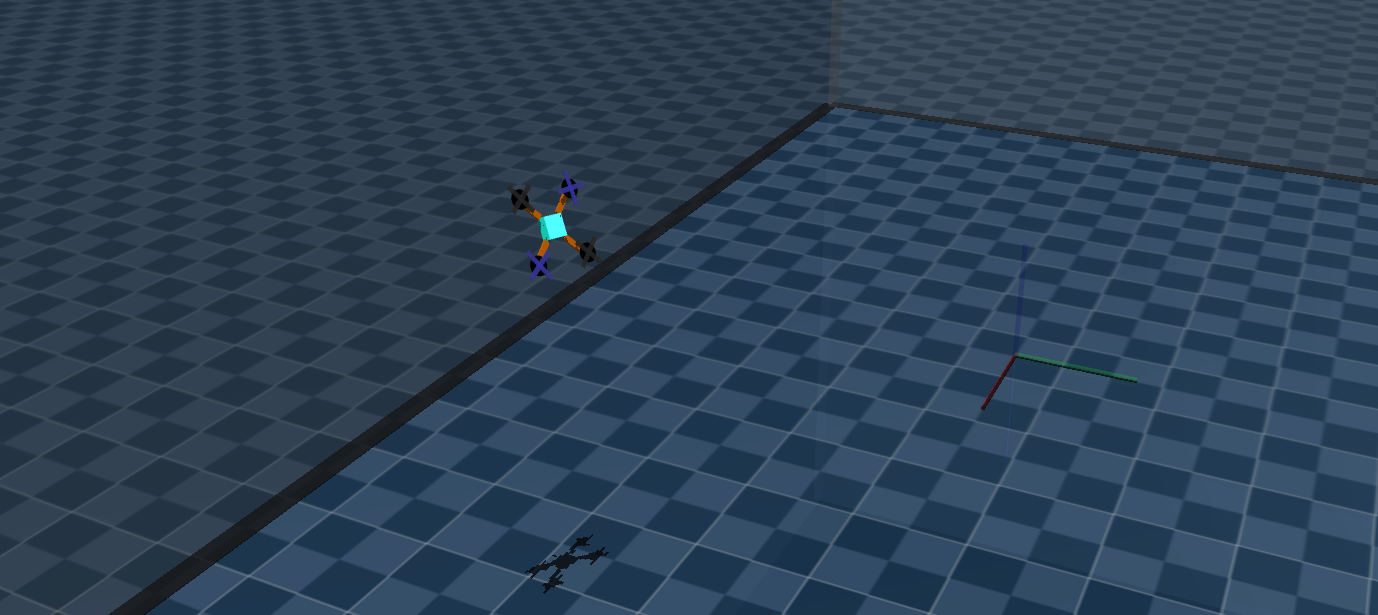
\includegraphics[width=\columnwidth]{figs/Mujuco_sim.png}
  \caption{\mujoco{} software-in-the-loop environment.  The quadrotor
           (m\,=\,\SI{1.08}{\kg}) is simulated by \mujoco{}'s internal
           rigid-body integrator at \SI{500}{\hertz} while the body-rate
           \nmpc{} runs at \SI{100}{\hertz} and communicates with
           the simulator over ROS~2.  The gates (red rings) and the
           \pmm{}-optimal reference are rendered for visual reference;
           a random external-force disturbance re-drawn at every reset
           provides trial-to-trial stochasticity.}
  \label{fig:mujoco_sim}
\end{figure}

\subsection{Reference Configurations}
\label{sec:configurations}

Both configurations track $\vect{p}^*(t)$ and $\vect{v}^*(t)$ from the
\pmm{} output and use identical dynamics, solver, and cost structure;
the only variable is how much of the flatness reference is fed to the
tracker.
\nmpc{}-Att uses a yaw-only quaternion
$\vect{q}^*_\psi=[\cos(\psi^*/2),0,0,\sin(\psi^*/2)]^\top$ with no
angular-rate or thrust feedforward ($\vect{\omega}^*=\vect{0}$,
$T^*=0$, $\mat{Q}_\omega=\mat{0}$).
\nmpc{}-Full applies the complete flatness chain
(Section~\ref{sec:flat_map}), adding the tilt-corrected quaternion,
angular-rate reference, and thrust feedforward, with all cost terms
active including $\mat{Q}_\omega=\mathrm{diag}(0.5,0.5,0.5)$.

% ------------------------------------------------------------------
\subsection{Evaluation Circuits}
\label{sec:circuits}
% ------------------------------------------------------------------

We evaluate both controllers on two complementary reference circuits
(Fig.~\ref{fig:pmm_circuits}, Table~\ref{tab:circuits}) chosen to
probe opposite operating regimes of the flatness bridge.

\textbf{Figure-8 (moderate racing).}
Eight gates form two interlocked lobes in the $\pm X$ direction with
altitude alternation in $[1.0,2.5]$~m.
The starting gate is placed at the figure-8 crossover so that the
drone's initial rest-to-speed transient aligns with the sustained
flight direction, eliminating a cold-start artefact that would bias
the comparison.
The required body attitude remains inside the flat-yaw manifold
($z^*_{b,z}>0$ throughout), so both configurations are expected to
be physically capable of tracking the reference.

\textbf{Vertical loop (acrobatic).}
Nine gates trace a \emph{vertical} circular section in the $XZ$ plane
(radius $\approx\!2$~m, centred at $z=3$~m) whose apex at $z=5$~m
forces an \emph{inverted} body attitude.
At the apex, the planned specific-force vector points downward in the
world frame, so $z^*_{b,z}<0$ and the tilt-corrected quaternion
departs from the flat-yaw manifold.
The yaw-only reference
$\vect{q}^*_\psi=[\cos(\psi^*/2),0,0,\sin(\psi^*/2)]^\top$ used by
\nmpc{}-Att is \emph{structurally} unable to represent any attitude
with $z_{b,z}<0$ (since $R^*_{33}(\vect{q}^*_\psi)=+1$ for all
$\psi^*$), which turns this circuit into a feasibility test for the
complete flatness inversion.
The minimum observed $z^*_{b,z}=-0.97$ confirms the inversion
geometrically (Fig.~\ref{fig:pmm_circuits}(b)).

\begin{table}[!htbp]
  \centering
  \caption{PMM Solutions for the Two Evaluation Circuits.}
  \label{tab:circuits}
  \renewcommand{\arraystretch}{1.1}
  \begin{tabular}{lcc}
    \toprule
    & Figure-8 & Vertical Loop \\
    \midrule
    Gates ($N_g$)                          & 8                     & 9                     \\
    Arc length [\si{\m}]                   & 54.8                  & 31.9                  \\
    $T_f^*$ [\si{\s}]                      & 5.55                  & 5.40                  \\
    $v_\text{mean}$ [\si{\metre\per\second}] & 9.85                & 5.89                  \\
    $v_\text{peak}$ [\si{\metre\per\second}] & 16.55               & 12.10                 \\
    $z^*_{b,z,\min}$                        & $-0.34$              & $-0.97$ (inverted)    \\
    $\max|\vect{\omega}^*|$ [\si{\radian\per\second}] & 9.00 (clipped) & 9.00 (clipped)     \\
    $T^*$ range [\si{\N}]                   & $[5.8,\,42.4]$       & $[1.5,\,42.4]$        \\
    \bottomrule
  \end{tabular}
\end{table}

\begin{figure*}[!htbp]
  \centering
  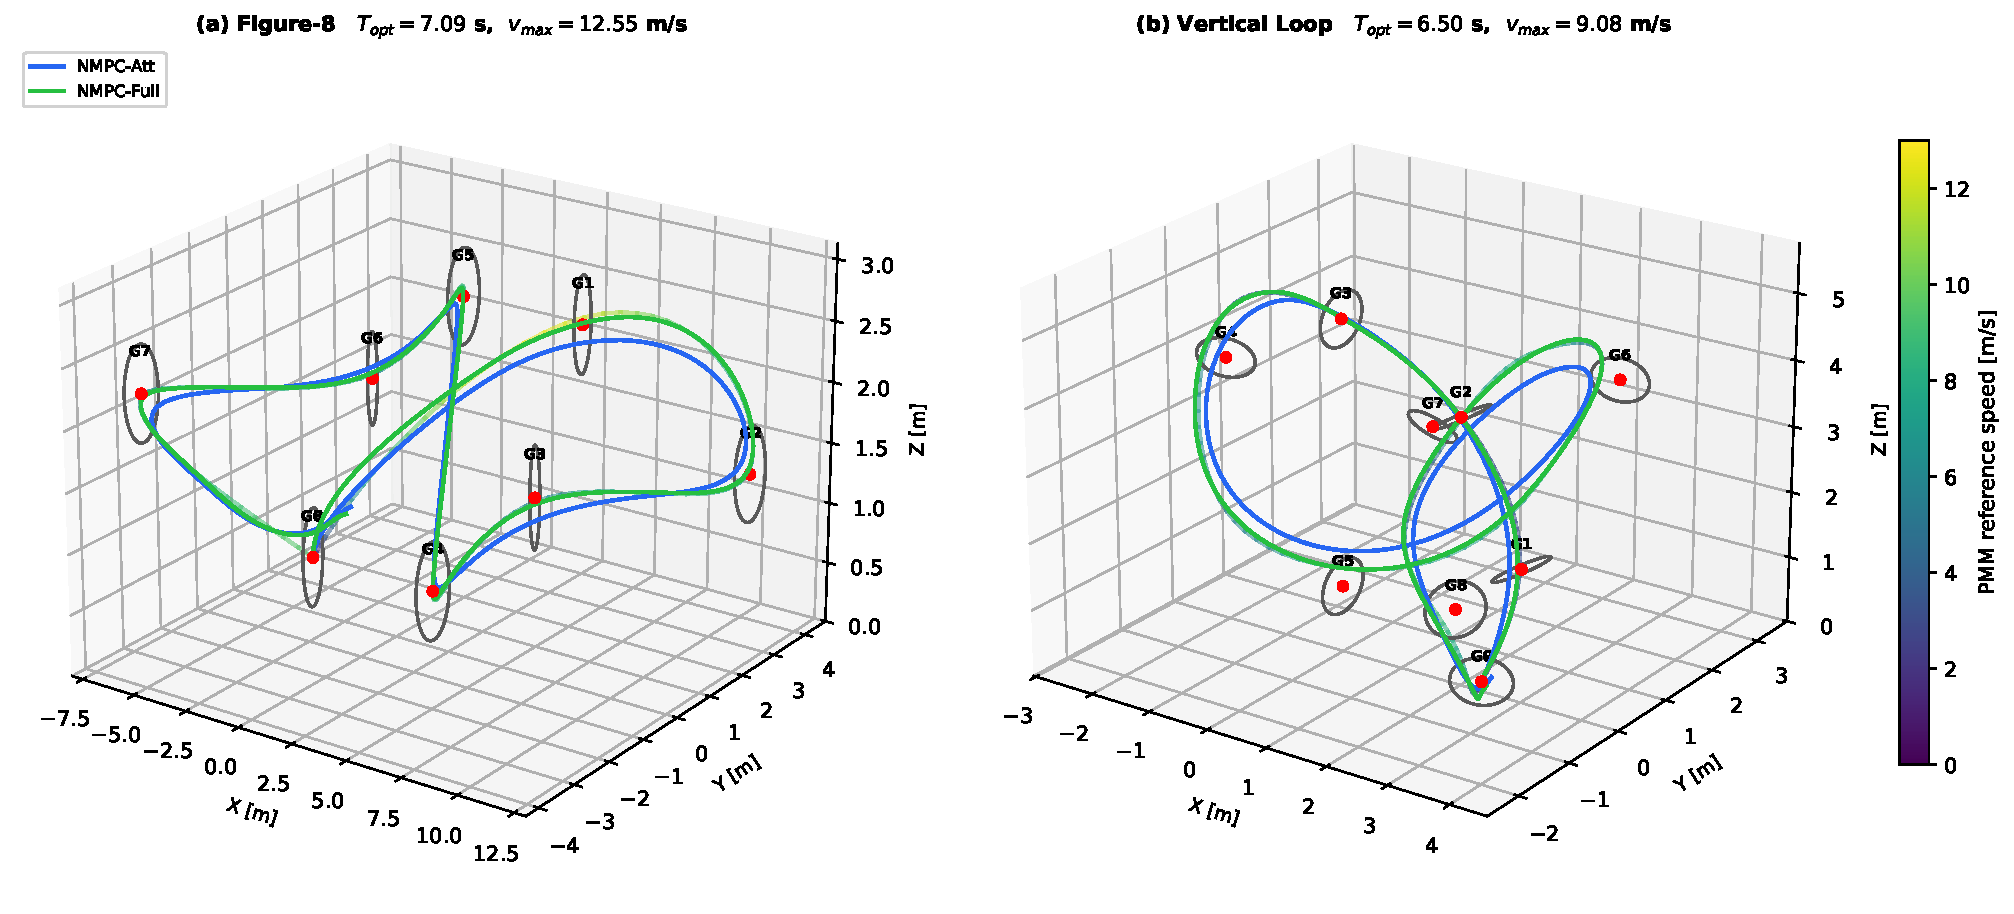
\includegraphics[width=\textwidth]{figs/fig_pmm_circuits.pdf}
  \caption{Evaluation circuits in 3-D.
           (a)~Figure-8: moderate racing reference with altitude
           alternation (crossover start eliminates the cold-start
           transient).
           (b)~Vertical loop: acrobatic reference whose apex (G3)
           forces an inverted body attitude ($z^*_{b,z}<0$),
           exceeding the representational range of any yaw-only
           attitude reference.
           Viridis-coloured line: \pmm{} reference coloured by
           instantaneous speed; blue: \nmpc{}-Att; green:
           \nmpc{}-Full; red markers: gate centres.}
  \label{fig:pmm_circuits}
\end{figure*}

Figure~\ref{fig:flatness_analysis_loop} confirms that the
flatness-derived feedforward is non-trivial on the acrobatic circuit:
angular rates reach the $\pm\SI{9}{\radian\per\second}$ saturation
clip in the loop and collective thrust drops to
$\approx\!\SI{3.3}{\N}$ at the inverted apex (near the theoretical
minimum for a circular orbit at $v^2/R\approx g$).
Both signals are identically zero in \nmpc{}-Att.

\begin{figure}[!htbp]
  \centering
  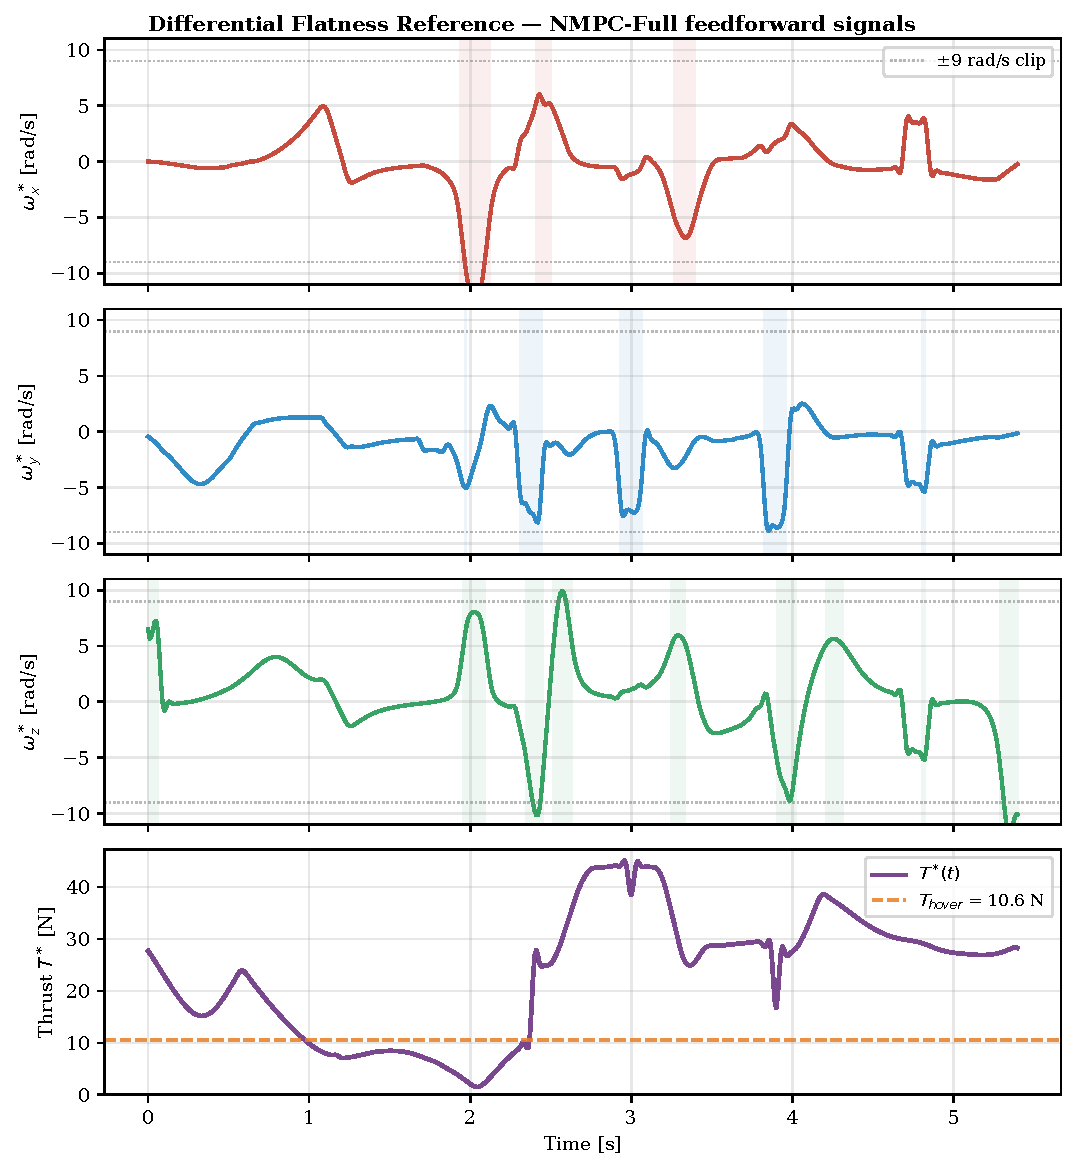
\includegraphics[width=\columnwidth]{figs/fig_flatness_analysis_loop.pdf}
  \caption{Flatness-derived feedforward on the vertical loop.
           \emph{Top three panels}: body angular-rate reference
           $\vect{\omega}^*(t)$ per axis (shaded:
           $|\omega_i^*|>\SI{5}{\radian\per\second}$; dotted:
           $\pm\SI{9}{\radian\per\second}$ clip).
           \emph{Bottom}: collective thrust $T^*(t)$ (purple) versus
           hover thrust $T_\text{hover}=mg=\SI{10.6}{\N}$.
           Thrust collapses to $\approx\!\SI{3.3}{\N}$ at the
           inverted apex. All four signals are zero in \nmpc{}-Att.}
  \label{fig:flatness_analysis_loop}
\end{figure}

% ------------------------------------------------------------------
\subsection{Tracking Performance}
\label{sec:tracking}
% ------------------------------------------------------------------

We run $N=25$ software-in-the-loop (SiL) trials per controller per
circuit against the \mujoco{} physics engine driven through ROS~2.
Stochasticity arises from the randomly seeded external-force
disturbance that MuJoCo re-draws at every scene reset, so each of
the 100 total trials is an independent realisation.
Trials in which either controller diverged ($\text{RMSE}>\SI{5}{\m}$,
\SIrange{5}{15}{\percent} per mode, attributable to the tail of the
disturbance distribution) are flagged as \emph{blow-ups} and excluded
from the statistics; we report the success rate alongside the
continuous metrics.
Table~\ref{tab:results} consolidates all four configurations with
mean $\pm$ standard deviation over valid trials.

\begin{table}[!htbp]
  \centering
  \caption{SiL Tracking Performance: Common-Practice Yaw Reference
           (\nmpc{}-Att) vs.\ Complete Flatness Inversion
           (\nmpc{}-Full) on Both Circuits ($N=25$ MuJoCo trials with
           random external-force disturbance; mean\,$\pm$\,std over
           valid trials; Gates: mean crossings per trial; bold\,=\,best).}
  \label{tab:results}
  \renewcommand{\arraystretch}{1.05}
  \scriptsize
  \resizebox{\columnwidth}{!}{%
    % auto-generated by experiments/stats_summary.py — do not edit by hand
\setlength{\tabcolsep}{2.5pt}
\begin{tabular}{@{}llcccc@{}}
  \toprule
  Circ. & Ctrl. & RMSE [\si{\m}] & Gates & $d_\mathrm{gate}$ [\si{\m}] & P99 [\si{\ms}] \\
  \midrule
  \multirow{2}{*}{Fig8}
    & Att  & $0.407 \pm 0.007$ & $3.09/7$ & $0.373 \pm 0.004$ & $4.39$ \\
    & Full & $\mathbf{0.308 \pm 0.007}$ & $\mathbf{7/7}$ & $\mathbf{0.146 \pm 0.004}$ & $3.86$ \\
  \midrule
  \multirow{2}{*}{Loop}
    & Att  & $0.289 \pm 0.007$ & $5/8$ & $0.300 \pm 0.003$ & $3.86$ \\
    & Full & $\mathbf{0.211 \pm 0.009}$ & $\mathbf{8/8}$ & $\mathbf{0.151 \pm 0.005}$ & $3.85$ \\
  \bottomrule
\end{tabular}
%
  }
\end{table}

\subsubsection{Figure-8 Circuit}

On the seven-gate figure-8 (peak speed
\SI{16.6}{\metre\per\second}, peak acceleration
\SI{36.3}{\metre\per\second\squared}), \nmpc{}-Full completes all
seven gates in every valid trial ($7/7$), while \nmpc{}-Att
crosses only $3.09/7$ on average (\SI{44.1}{\percent}).
\nmpc{}-Full reduces position RMSE by \SI{24.3}{\percent}
(\SI{0.407}{\m}~$\to$~\SI{0.308}{\m}) and mean gate-crossing
distance by \SI{60.8}{\percent}
(\SI{0.373}{\m}~$\to$~\SI{0.146}{\m}).
Figure~\ref{fig:pmm_circuits}(a) and Fig.~\ref{fig:pos_error}
visualise the gap as a consistent offset concentrated around gate
transitions, produced by the yaw-only attitude reference fighting
the horizontal-thrust tilt the aggressive PMM trajectory demands.

\subsubsection{Vertical Loop}

On the eight-gate loop (peak speed \SI{12.1}{\metre\per\second},
peak acceleration \SI{33.8}{\metre\per\second\squared}), the
categorical separation is even sharper: \nmpc{}-Full completes
$8/8$ gates in every valid trial, whereas \nmpc{}-Att averages
only $5/8$ (\SI{62.5}{\percent}); the missed gates cluster around
the inverted apex (G2--G5), which the yaw-only reference cannot
represent by construction ($R^*_{33}(\vect{q}^*_\psi)=+1$ for all
$\psi^*$).
\nmpc{}-Full reduces position RMSE by \SI{27.2}{\percent}
(\SI{0.289}{\m}~$\to$~\SI{0.211}{\m}) and mean gate-crossing distance
by \SI{49.6}{\percent}
(\SI{0.300}{\m}~$\to$~\SI{0.151}{\m}).
The attitude-feasibility argument is structural: no choice of cost
weights can drive \nmpc{}-Att to an attitude with $z_{b,z}<0$, so the
deficit is inherent to the reference, not an artefact of tuning.
Figure~\ref{fig:gate_error_loop} shows that \nmpc{}-Att exceeds the
gate radius precisely at the inverted section, while \nmpc{}-Full
stays inside at every gate.
Together, the two circuits isolate \emph{what gains can fix}
(figure-8, a quantitative gap) from \emph{what only reference
enrichment can fix} (loop, a categorical gap).

\begin{figure}[!htbp]
  \centering
  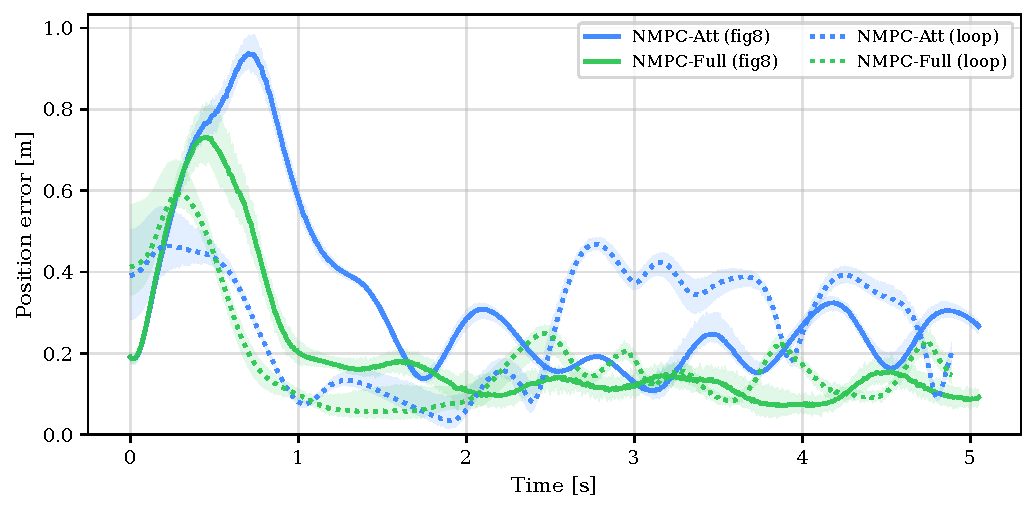
\includegraphics[width=\columnwidth]{figs/fig_pos_error_combined.pdf}
  \caption{Position error norm
           $\norm{\vect{p}(t)-\vect{p}^*(t)}$ on both circuits
           (fig-8: solid; loop: dashed).
           In the figure-8, \nmpc{}-Full stays consistently below
           \nmpc{}-Att with peaks at gate-crossing instants.
           In the vertical loop, \nmpc{}-Att diverges during the
           inverted-apex traversal
           ($t\!\approx\!2.5$--$4.5$~\si{\second});
           \nmpc{}-Full tracks the reference throughout.}
  \label{fig:pos_error}
\end{figure}

\begin{figure}[!htbp]
  \centering
  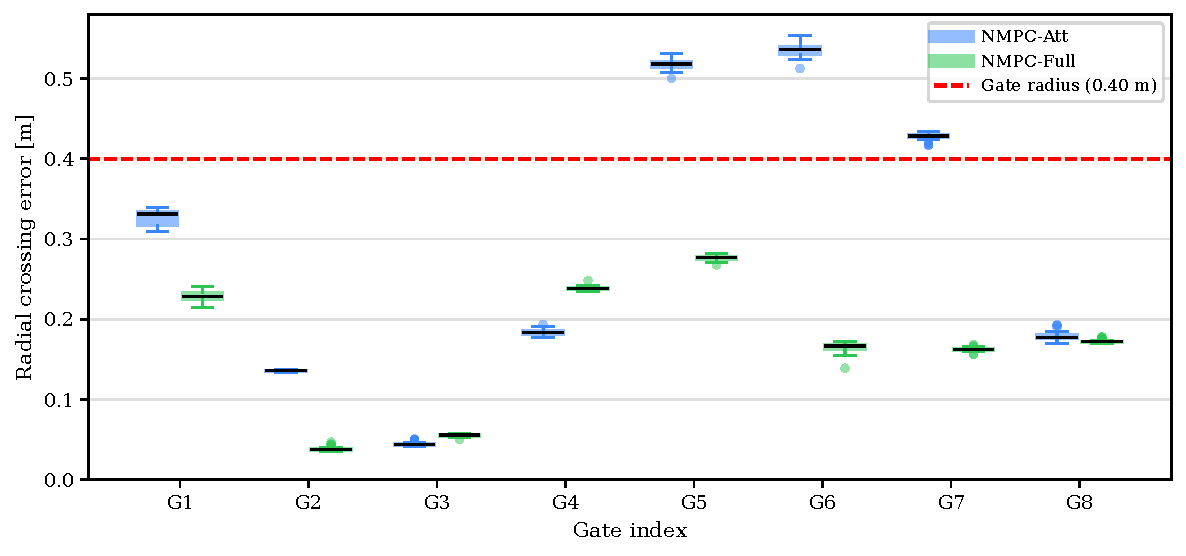
\includegraphics[width=\columnwidth]{figs/fig3_gate_error_loop.pdf}
  \caption{Vertical loop: minimum 3-D distance to each gate centre,
           aggregated as a box plot over the 18 valid SiL trials per
           controller.
           Dashed line: gate radius $r=\SI{0.4}{\m}$.
           \nmpc{}-Att exceeds the radius at gates G2--G5 (inverted
           section); \nmpc{}-Full remains below $r$ at every gate.}
  \label{fig:gate_error_loop}
\end{figure}

% ------------------------------------------------------------------
\subsection{Mechanism: Attitude and Rate Tracking}
\label{sec:mechanism}
% ------------------------------------------------------------------

Figure~\ref{fig:att_error_loop} resolves the mechanism at the
attitude level.
The \nmpc{}-Att attitude error exceeds \SI{90}{\degree} during the
inverted section because the reference it is following
($\vect{q}^*_\psi$) is geometrically the wrong attitude --- the
target is at the antipode of the feasible tilt, and no amount of
feedback gain can recover it.
\nmpc{}-Full receives the correct tilt-corrected reference and its
error stays bounded.

\begin{figure}[!htbp]
  \centering
  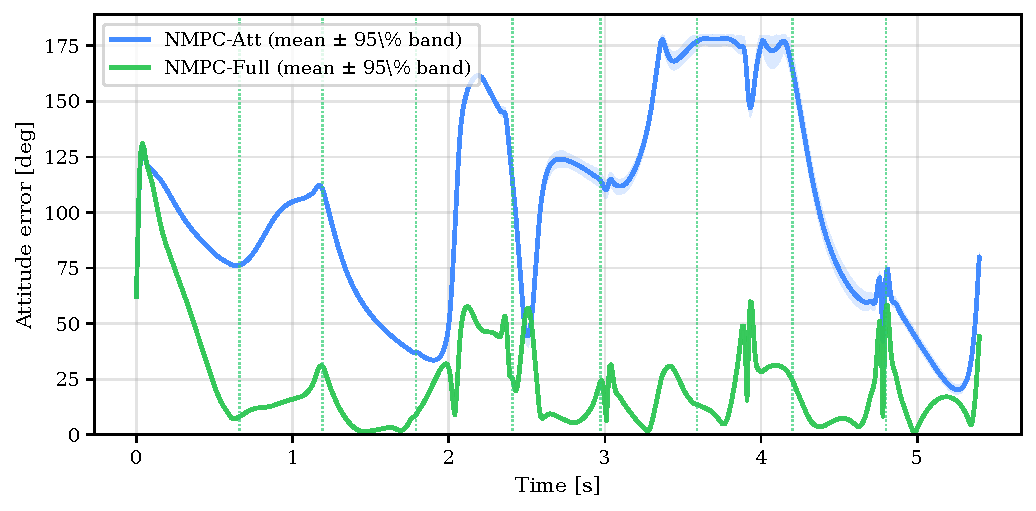
\includegraphics[width=\columnwidth]{figs/fig6_att_error_loop.pdf}
  \caption{Vertical loop: attitude error
           $\|\log(\mat{R}\mat{R}^{*\top})\|_F$ in degrees.
           \nmpc{}-Att diverges at the apex because
           $\vect{q}^*_\psi$ cannot represent the inverted attitude;
           \nmpc{}-Full tracks the flatness-derived reference with
           bounded error.}
  \label{fig:att_error_loop}
\end{figure}

% ------------------------------------------------------------------
\subsection{Computational Performance}
\label{sec:computation}
% ------------------------------------------------------------------

Reference enrichment carries \emph{no} computational penalty.
Both configurations share identical OCP dimensions and differ only
in weight values and parameter content, so solver work per step is
invariant.
Across both circuits and all 82 valid SiL trials, P99 solve time
stays below \SI{4.4}{\milli\second}, giving $>\!2\times$ margin to
the \SI{10}{\milli\second} \nmpc{} deadline
(Table~\ref{tab:results}, last column).
Hence the categorical feasibility gain on the loop and the
\SIrange{24}{27}{\percent} RMSE reduction on both circuits are
delivered with zero trade-off against real-time budget.

% ------------------------------------------------------------------
\subsection{Discussion}
\label{sec:discussion}
% ------------------------------------------------------------------

The two circuits split the contribution of the full flatness
inversion into two distinct claims.

\emph{Quantitative, in the flat-yaw regime.}
On the figure-8, where the yaw-only reference is at least
geometrically feasible, \nmpc{}-Full reduces position RMSE by
\SI{24.3}{\percent} and more than halves the mean gate-crossing
distance (\SI{60.8}{\percent}), at identical solver cost.
This isolates the value of the angular-rate and thrust feedforward:
without them, the tracker must infer the required body tilt from
error feedback and absorbs a controller-cycle lag at every
acceleration transition, which at \SI{16.6}{\metre\per\second} peak
speed pushes the mean crossing distance beyond the gate radius and
collapses the crossing rate of \nmpc{}-Att to \SI{44.1}{\percent}.

\emph{Categorical, in the non-flat regime.}
On the vertical loop, the yaw-only reference is geometrically
\emph{wrong} --- its third rotation column is always $+e_3$, while
the circuit requires $-e_3$ at the apex.
No choice of cost weights can fix this; only reference enrichment
does.
This is the stronger answer to the interface question of
Song~\textit{et~al.}~\cite{song2023reaching}: the limiting factor
of the \emph{planner--controller interface} is not its modular
architecture but the \emph{representational completeness} of the
reference passed across it.
Enriching the interface with the flatness output closes both the
quantitative and the categorical gap with no additional compute.

Two limitations qualify the scope.
The SiL experiment includes \mujoco{}'s random external-force
disturbance (re-drawn at every reset) and round-trip ROS~2 messaging,
but does not cover communication latency beyond the ROS~2 loopback
or aerodynamic effects such as rotor wash and drag, leaving full
sim-to-real robustness unquantified.
A learning-augmented controller that infers the flatness
feedforward from rollouts could in principle bridge the figure-8
gap, but the loop result suggests that \emph{reference completeness},
not controller capacity, is the binding constraint for acrobatic
flight.

% ==========================================================================
\section{Conclusion}
\label{sec:conclusion}
% ==========================================================================

This paper presented a hierarchical planning and control
framework for time-optimal agile gate navigation with quadrotor UAVs.
A Point Mass Model planner generates a time-optimal reference trajectory
offline; a differential flatness bridge maps this reference to the full
quadrotor state; and an SQP-RTI \nmpc{} tracks the converted reference
in real time at \SI{100}{\hertz}.
Two reference configurations were evaluated in \mujoco{} physics-engine
simulation to isolate the value of the flatness inversion.
\nmpc{}-Att, representing common practice, derives a yaw-only quaternion
from the velocity direction and includes no angular-rate or thrust
feedforward; its cost correctly omits the angular-rate penalty to avoid
contradictory objectives.
\nmpc{}-Full applies the complete flatness chain, providing the
tilt-corrected quaternion, angular-rate, and thrust feedforward with all
cost terms active.
Validation was performed in a software-in-the-loop setup driving
\mujoco{} through ROS~2 with a random external-force disturbance
re-drawn at every reset; $N=25$ trials were run per circuit per
controller under a consistent \SI{4}{g} thrust envelope shared by
planner and tracker.
On the seven-gate figure-8 (peak speed \SI{16.6}{\metre\per\second})
and the eight-gate vertical loop (peak speed
\SI{12.1}{\metre\per\second}), \nmpc{}-Full achieves
\SI{100}{\percent} gate-crossing in every valid trial, while
\nmpc{}-Att completes only \SI{44.1}{\percent} (fig-8) and
\SI{62.5}{\percent} (loop).
\nmpc{}-Full reduces position RMSE by \SI{24.3}{\percent} (fig-8)
and \SI{27.2}{\percent} (loop) and mean gate-crossing distance by
\SI{60.8}{\percent} and \SI{49.6}{\percent} respectively, while the
solver P99 time remains below \SI{4.4}{\milli\second} for both
configurations.
The figure-8 gap is quantitative --- driven by the missing
angular-rate and thrust feedforward at sharp acceleration
transitions --- whereas the loop gap is categorical: the yaw-only
reference cannot represent the inverted attitude at the apex, so
only reference enrichment closes it.
Ongoing work extends the validation to hardware-in-the-loop with
realistic communication latencies and aerodynamic effects, and to
deployment on a physical quadrotor platform to quantify the
sim-to-real gap.

\bibliographystyle{IEEEtran}
\bibliography{references}

% \begin{IEEEbiography}[{
\includegraphics[width=1in,height=1.25in,clip,
% keepaspectratio]{author1.png}}]{Bryan S. Guevara}
% received the B.Sc. degree in mechatronics engineering. He is currently
% pursuing the Ph.D. degree at the Laboratório de Automação e Sistemas de
% Robótica (LaSER), Universidade Federal da Paraíba (UFPB), Brazil. His
% research interests include nonlinear model predictive control and agile
% autonomous UAV flight.
% \end{IEEEbiography}

% \begin{IEEEbiography}[{
\includegraphics[width=1in,height=1.25in,clip,
% keepaspectratio]{author2.png}}]{Luis F. Simancas}
% received the Ph.D. degree in control engineering. He is a researcher at
% the Instituto de Automática (INAUT), Universidad Nacional de San
% Juan--CONICET, Argentina. His research interests include optimal control
% and motion planning for robotic systems.
% \end{IEEEbiography}

% \begin{IEEEbiography}[{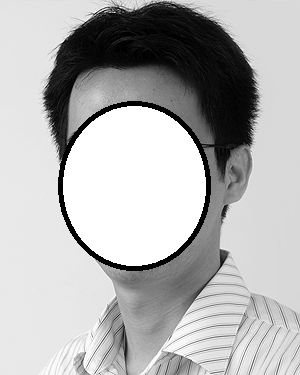
\includegraphics[width=1in,height=1.25in,clip,
% keepaspectratio]{author3.png}}]{Tiago Nascimento}
% (Member, IEEE) received the Ph.D. degree in robotics. He is a Professor
% at the Laboratório de Automação e Sistemas de Robótica (LaSER),
% Universidade Federal da Paraíba (UFPB), Brazil. His research interests
% include autonomous UAVs, multi-robot systems, and human-robot
% interaction.
% \end{IEEEbiography}

\EOD

\end{document}
